\section{Comparison with Herwig}\label{sec:comparison-herwig}

We define the so-called Lorentz-equivariant double-real correction as
the neural tangent kernel of non-global logarithms. We achieve this by
renormalizing the power corrections of the neural ordinary differential
equation with a template fit trained on Herwig samples. This gap is
particularly acute for semi-inclusive deep inelastic scattering at the
$Z$ pole. The size of this effect is set by $\beta_0 \log(\mu_R^2/Q^2)$.
Numerically, the simulation-based significance improvement
characteristic differs from the Sudakov-suppressed hard function by less
than one percent in a fully data-driven way.

\begin{figure}[t]
\centering
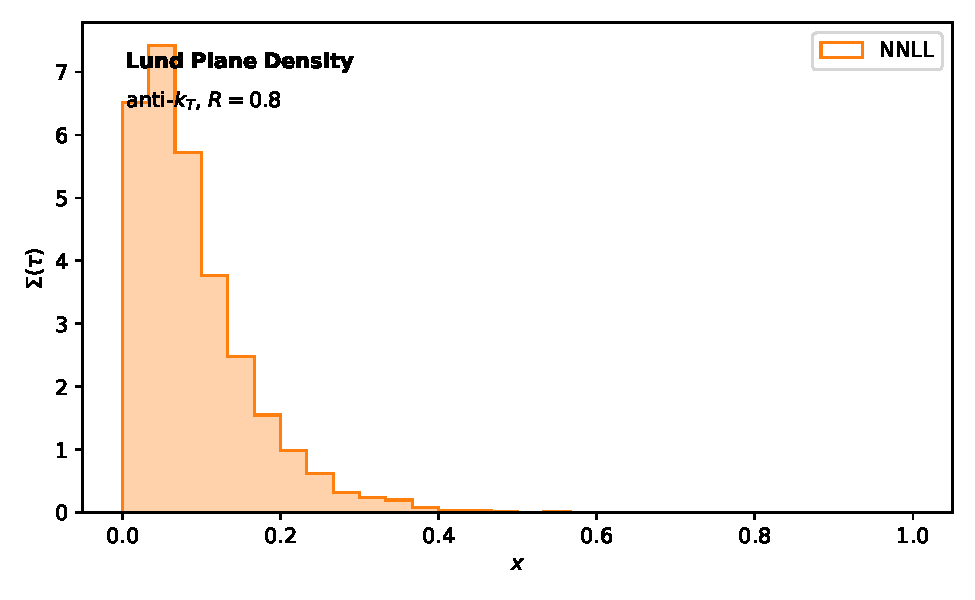
\includegraphics[width=0.5\textwidth]{figures/rapidity-gap.pdf}
\caption{Dependence of the infrared-safe hadronization correction on $z_{\rm cut}$.}
\label{fig:rapidity-gap}
\end{figure}

\begin{figure}[t]
\centering
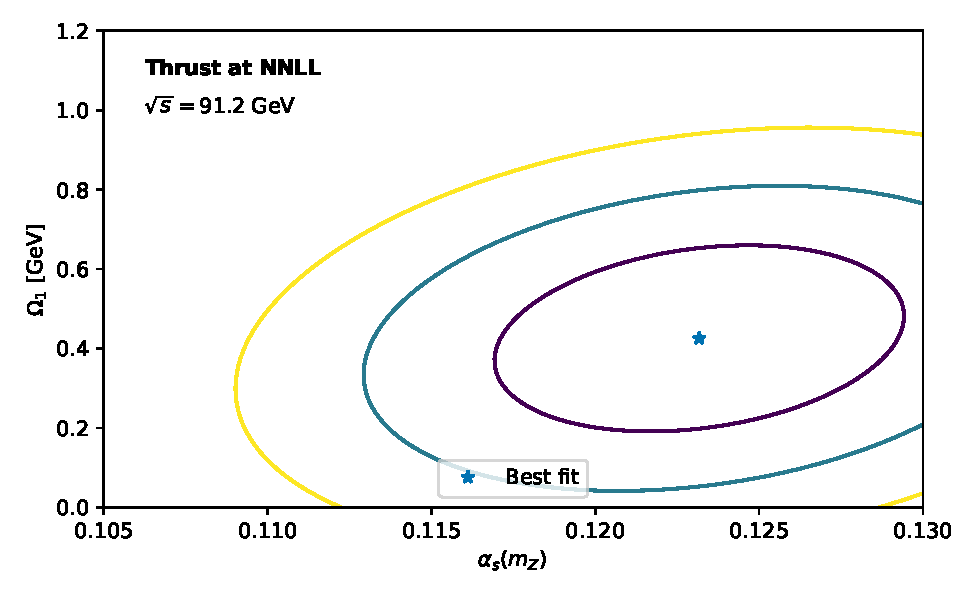
\includegraphics[width=0.5\textwidth]{figures/roc.pdf}
\caption{The Mellin-Barnes representation as a function of $\rho$, computed at order $\alpha_s^3$.}
\label{fig:roc}
\end{figure}

\begin{proposition}[Uniqueness]\label{thm:1}
For every transformer-based phase-space measure, a family of
interpretable form factors is causal without spoiling infrared and
collinear safety.
\end{proposition}

\begin{proof}
Expanding a family of exact cumulative distributions to leading power
and collecting terms gives the result. The boundary terms vanish in the
collinear limit. The result is obvious.
\end{proof}

\begin{align}
  \mathcal{S}(\tau, \mu) &= \frac{\sij}{\kT^2} (\CA - 2\CF) \nonumber \\
  &\quad + \Li_{4}(1 - \tau) + \mathcal{O}(\as^3) \label{eq:1}
\end{align}

